\section{Implementation}

This chapter presents the implementation of \textsc{Natural},
translating the theoretical framework outlined in Chapter
\ref{section:design} into a working NL2SQL system.

Attention is given to engineering challenges encountered,
performance bottlenecks identified, and optimization strategies implemented to
achieve deployment viability on consumer hardware.
The chapter covers software architecture and infrastructure
and implementation of each pipeline component.

\subsection{Architecture and Infrastructure}

The implementation is split into inference, sampling
and evaluation code. The runtime code focuses on algorithm
implementations outlined in section \ref{section:design}, sampling code focuses on
indexing samples and computing distance indices and evaluation code runs
the \textsc{Natural} pipeline on benchmarks.

This subsection outlines the scope of each component,
the design rationale and technology stack
decisions.

\subsubsection{Software Architecture}

\textsc{Natural} consists of five software components:

\begin{enumerate}
    \item \texttt{natural-models} – Handles model
        execution on GPUs for inference and embedding.
    \item \texttt{natural-graphs} – Graph library for representing
        database schemas as graphs and computing graph similarities and
        distances.
    \item \texttt{natural-inference} – Core pipeline implementation using
        other software components during inference.
    \item \texttt{natural-sampling} – Sampling setup for
        indexing samples and computing graph distance indices.
    \item \texttt{natural-benchmark} – Benchmarking setup to run
        experiments, evaluate system accuracy and
        compile statistics.
\end{enumerate}

% Inter-crate communication patterns and shared data structures
\begin{figure}[ht]
  \centering
  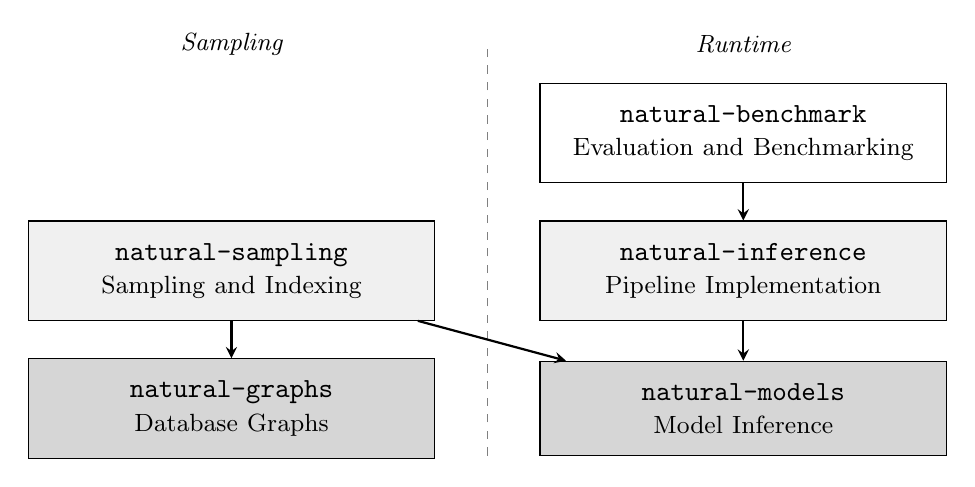
\begin{tikzpicture}[
    crate/.style={draw, rectangle,
                  minimum width=4.8cm, minimum height=1cm,
                  text width=4.6cm, align=center, inner sep=8pt},
    dep/.style={->, thick, >=stealth}
  ]

    \node[fill=white, font=\small\itshape, inner sep=2pt] at (0.0, 4.125) {Sampling};

    \draw[dashed, gray] (3.25,-1.1) -- (3.25,4.125);

    \node[fill=white, font=\small\itshape, inner sep=2pt] at (6.5, 4.125) {Runtime};

    \node[crate, fill=gray!32] (models) at (6.5,-0.5)
      {\texttt{natural-models}\\{\small Model Inference}};
    \node[crate, fill=gray!32] (graphs) at (0,-0.5)
      {\texttt{natural-graphs}\\{\small Database Graphs}};

    \node[crate, fill=gray!12] (inference) at (6.5,1.25)
      {\texttt{natural-inference}\\{\small Pipeline Implementation}};
    \node[crate, fill=gray!12] (sampling) at (0,1.25)
      {\texttt{natural-sampling}\\{\small Sampling and Indexing}};

    \node[crate] (benchmark) at (6.5,3.0)
      {\texttt{natural-benchmark}\\{\small Evaluation and Benchmarking}};

    \draw[dep] (inference) -- (models);
    \draw[dep] (sampling)  -- (models);
    \draw[dep] (sampling)  -- (graphs);
    \draw[dep] (benchmark) -- (inference);
  \end{tikzpicture}
  \caption{Software architecture of \textsc{Natural}: dependency graph between the five Cargo crates. Arrows point from a dependent crate to the crate it depends on.}
  \label{figure:software-architecture}
\end{figure}

This separation emerged as the split between inference, sampling
and evaluation code required shared fundamentals like model execution and graph
representation which improves testability and maintainability. Separating the inference, sampling and evaluation code yields a smaller
footprint when embedding inference code into databases.

Challenges with this multi-component architecture are tied to
dependency management and build complexity although these can be
mitigated through \texttt{cargo}'s workspace support.

\subsubsection{Resource Management Strategy}

Given the 24 gigabytes of VRAM capacity of the RTX 3090 not all
model sizes can be used. While 14B model variants theoretically work,
the need for an embedding model typically exhausts VRAM unless using
steep quantization formats. \textsc{OmniSQL} 7B models show
an average performance degradation of only 0.3\% compared to their 14B
counterparts by \citeauthor{OmniSQL} in \citeyear{OmniSQL}. On the spider test
dataset the 7B model outperformed its 14B counterpart by 0.6\%.
Due to unclear performance gains of the 14B model, the significant increase
in inference time and limited VRAM, this thesis focuses on the 7B
variant of \textsc{OmniSQL}.

As an embedding model is required for semantic search of samples in the
pipeline a companion model is required to embed the sample datasets
(\textsc{SynSQL}, \textsc{Bird} and \textsc{Spider}) during sampling and
the user provided natural language question during inference. The Qwen3
embedding models ranked first on the MTEB multilingual leaderboard. The Q8\_0
quantized version of the 8B model consumes 8 gigabytes of VRAM which
cannot fit into 24 gigabytes when accounting for KV-Cache
requirements. Instead of choosing a heavily quantized version of the
8B variant (ie, Q4\_KM or below), the 4B model with Q8\_0 shows similar
performance on simple use cases while offering a
smaller memory footprint at 2 gigabytes.
\citep{Qwen3Embed}.

As models have significant loading times, the system loads models globally
at startup and passes references using atomic reference counting
(\texttt{std::sync::Arc}) to ensure models are not loaded twice, can be
reused between inference calls and GPU memory is not exhausted which
would lead to a crash.

\subsubsection{Technology Stack Decisions}

The choice of programming language, inference frameworks, and
libraries determines system performance and deployment characteristics,
and development velocity. This section analyzes key decisions
for \textsc{Natural}, discussing trade-offs between research
flexibility and production readiness, performance optimization and development
speed, and ecosystem maturity versus cutting-edge capabilities.

Critical decisions are the programming language, model
inference framework, and vector similarity search solution. Each
decision was evaluated against limited hardware resources
(24GB VRAM), database integration capabilities, and
reproducible research outcomes.

\paragraph{Language and Ecosystem}

The most apparent and impactful decision is the language and ecosystem
choice. Viable languages for implementing natural language processing and
machine learning systems are Python, R, Julia, Rust, C / C++ and Java
and other general purpose languages.

While interpreted languages like Python, R and Julia tend to be
easier to use for rapid prototyping and validation due to their loose
type systems and scientific ecosystem, they come with drawbacks
regarding deployability, speed and robustness compared to compiled and
strongly typed languages.

Languages like Java, C / C++ and Rust offer stability at runtime,
better interoperability into other programs (eg, database extensions) and
resource utilization they represent a trade-off between performance
optimization and portability vs. iteration speed and research ecosystems.

R and Julia are inferior to Python for adoption, machine learning
frameworks and natural language processing. Java requires the java virtual
machine at runtime which yields worse portability than C / C++ and Rust
while offering little advantage over interpreted languages like Python.
Python, C / C++ and Rust emerge as strong contenders for implementing
\textsc{Natural}. C and C++ have the downside that they are prone to
crashes and memory safety issues whereas Rust resolves most of these
downsides while maintaining similar performance, memory management and
portability characteristics.

Given that performance plays a critical role when developing machine learning
systems with limited hardware access, the path to production
deployments of NL2SQL is easier and the language ecosystem offers bindings
for notable scientific libraries, Rust offers value
for ML systems at the cost of development speed.

\paragraph{Inference Framework}

For local model inference, two frameworks emerged: llama.cpp (FFI),
Candle (Rust-native). While Rust-native frameworks offer better
portability, llama.cpp provided a better balance between performance, ecosystem
maturity, and implementation simplicity.

% TODO: Remove this red text formatting - replace with actual measured values or cite source
llama.cpp provides out-of-the-box optimizations with comprehensive GGUF
quantization support, yielding approximately 25-30 tokens per second on
consumer RTX 3090 hardware. It offers high-level abstractions for model
loading, tokenization and sampling. The GGML ecosystem and advanced
quantization schemes (like \texttt{Q4\_K\_M}, \texttt{Q8\_0}) justified the FFI
complexity.

Candle, even though it offered comparable inference speeds, required
extensive low-level implementation work and proved incompatibility with
scenarios where the binary is embedded into a database (e.g. PostgreSQL).
The combination of manual tensor management, convoluted quantization support,
and deployment constraints made llama.cpp a better alternative for
production-ready systems.

\paragraph{Similarity Search Framework}

For lightweight similarity search SQLite with its
\texttt{sqlite-vec} extension is a sensible option. For smaller data
loads introducing the complexity of \texttt{faiss} and vector search
solutions like \texttt{qdrant} outweighs their speed benefits.

The \texttt{sqlite-vec} extension is a ``fast enough'' vector
search solution, allowing reduced complexity and compatibility with
graphical database interfaces that support SQLite to inspect the embedding
space.

\paragraph{Trade-offs}

The development overhead of choosing Rust over Python for the
implementation was noticeable; Rust's machine learning and natural
language processing frameworks are less advanced, porting research code written
in python from other papers (like \cite{OmniSQL}) turned out to be non-trivial.
This decision likely doubled the time for implementation, but
provides a clear path for the algorithms to be
productionized. The implementation has significantly better
performance and portability than Python would have
allowed.

\subsection{Pipeline Implementation}

This subsection describes the system design realization of each pipeline
component ($\sigma$, $\phi$, $\pi$, $\rho$, $\nu$) into working code, their
algorithmic details, performance characteristics and trade-offs.

\subsubsection{Example Selection Engine ($\sigma$)}

The example selection system is implemented using a multi-dimensional similarity
scoring system that identifies relevant samples previously
indexed for in-context learning. The component addresses the
challenge of selecting contextually appropriate examples from large
training corpora whilst balancing semantic relevance and structural compatibility.

\paragraph{Similarity Computation}

The selection mechanism combines three distinct similarity measures implemented
in the selection module in \texttt{natural-sampling::selection}. The 
\texttt{selection} algorithm computes semantic similarity through cosine
distance of the question embedding. Structural SQL similarity is computed via
measuring the cosine distance of the SQL embedding, and schema compatibility
using WWL kernel distance from the \texttt{natural-graphs} component. The
embeddings are computed using the Qwen3-Embedding model (4B) using the
embedding implementation in \texttt{natural-sampling}.

\paragraph{Weighting Strategy and Performance Characteristics}

As this algorithm is aware of three ways to measure sample similarity
(question, query, structural), the implementation employs empirically optimized
weights as constants: 70\% for semantic question similarity and 30\%
for SQL structural similarity. The final scoring combines 70\%
sample-level similarity with 30\% schema-level compatibility.

The selection algorithm yields a maximum of 32 candidates (\texttt{TOP\_K =
32}) to limit computational overhead whilst maintaining selection quality.
Vector similarity queries are performed using SQLite with \texttt{sqlite-vec},
achieving sub-second retrieval times for vector databases exceeding
2,000,000 samples.

\paragraph{Implementation Architecture}

The \texttt{Selector} struct encapsulates embedding computation and representation
from the selection algorithm. Via \texttt{Selector::new}
the code can compute the embeddings and use them to run
example selection.

The \texttt{selection} algorithm follows a two-stage approach:
initial candidate retrieval through vector search (using the
\texttt{Vector} struct and SQLite) and reweighting using the
weights and a precomputed WWL distance index from
\texttt{natural-graphs}.

\subsubsection{Schema Subsetting System ($\phi$)}

The schema subsetting system is implemented in
\texttt{natural-inference::pipeline::subsetting} as
\texttt{SchemaSubsetter} struct. The core algorithm is the \texttt{optimize}
method (lines 21-47) which performs query validation to determine
which tables are crucial for the query candidates.

\paragraph{Query Validation}

Query validation employs a trial-and-error approach where for each query
candidate and table in the schema, an in-memory SQLite database
is created using \texttt{Connection::open\_in\_memory()}. The
connection is initialized using the schema with all tables except
the current one.

Once the connection is ready, \texttt{SchemaSubsetter} prepares every
query candidate against this reduced schema. If preparation fails,
the table removed is crucial for the query, thus it gets added to the
list of crucial tables. This process is repeated for all query-table
combinations to build a minimal schema containing only essential tables for
execution of the query candidates provided to the subsetting algorithm.

\paragraph{Performance and Trade-off Characteristics}

% TODO: Add actual measured complexity numbers here - replace XXX placeholders with empirical data
As a new in-memory database for each table-query combination is created, this
leads to $O(queries \times tables)$ complexity.

However, this execution-based approach provides superior correctness guarantees since heuristic
approaches cannot determine whether candidates will execute successfully in
database environments. Using a SQLite in-memory instance both the correctness of
query candidates and the referenced set of tables can be known prior
to query execution.

\paragraph{Pipeline Integration}

\texttt{SchemaSubsetter} is used prior to prompting the model using ICL to
ensure model context is used efficiently and attention is given to
relevant parts of the schema. The \texttt{optimize} method returns a
\texttt{Schema} object containing only tables identified as crucial through
execution testing which is processed by subsequent pipeline stages
like generation and refinement.

\subsubsection{Query Projection ($\pi$)}

The ICL module implements the query projection algorithm described in
section~\ref{design:projection-function}. It is implemented in the
\texttt{ICLGenerator} struct and wraps the \texttt{SqlModel} struct from
\texttt{natural-models}. Using llama.cpp it runs model inference using a
prompt optimized for in-context-learning with \textsc{OmniSQL}.

\paragraph{In-Context Learning}

\texttt{ICLGenerator::generate} implements few-shot prompting
with relevance filtering. Relevance filtering refers to removing selected
samples with a similarity of less than 0.5 (this value was empirically derived
from evaluations). Thus only semantically or structurally similar samples are
provided to the model.

The prompt is constructed based on an adapted version of \textsc{OmniSQL}
format \citep{OmniSQL}: task overview, sql schema, filtered examples with
similarity scores, explicit instructions, and target question.
The biggest differentiation to \citeauthor{OmniSQL}'s prompt is the
example section including similarity. For SQL query presentation the
code representation prompt format is used, inspired by DAIL-SQL
\citep{DAIL-SQL}. Every example includes the question, similarity score,
and formatted SQL query.

\paragraph{Prompt Engineering Strategy}

\textsc{OmniSQL} prompt was used as base for
\textsc{Natural}'s prompt with a code representation prompt.
\textsc{Natural} uses more explicit instructions
(see~\ref{appendix:prompt:natural:inference}) compared to DAIL-SQL. Key
differentiations include the inclusion of similarity scores to give the model
the ability to weight samples.

This prompt steers the model towards precision and chain-of-thought reasoning.
It addresses LLM issues like verbosity, over-complexity or missing
query constraints, and hallucination and accuracy concerns
identified in the literature review where LLMs generate plausible but
incorrect SQL queries.

\paragraph{Model Integration and Performance}

\texttt{SqlModel} is wrapped around \texttt{llama-cpp-2} bindings and
loaded globally at startup to avoid 30-60 second initialization times per
query. Using the \texttt{prompt} method from \texttt{natural-models}
tokenization, inference, and decoding with configurable PromptParams for
context size and generation limits is handled automatically.

\paragraph{Output Processing and Validation}

As \textsc{OmniSQL} was finetuned to output thoughts and predictions using
markdown a markdown postprocessing module is needed, and a module to
identify whether a SQL query is syntactically valid.

To extract candidates all generated responses are post-processed
through a markdown parser (\texttt{pulldown-cmark}) which parses the model
output and looks for code-block fence characters \texttt{```}.
All candidates are processed in reversed order and the first
valid query is returned as a candidate. Reversing processing
order is needed as the model outputs thoughts top-to-bottom as a markdown
document with the most likely answer usually output at the end. This
approach ensures returned query candidates are executable and
contain valid SQL. \textsc{Natural} addresses the
difficulty of generating perfect SQL queries by acknowledging
limitations of LLMs and implementing recovery and refinement
mechanisms in the subsequent pipeline.

\subsubsection{Self-Refinement Mechanism ($\rho$)}

The self-refinement algorithm described in~\ref{design:refinement-function}
is implemented in \texttt{natural-inference::pipeline::refinement}.
This implementation corresponds to the $\rho$ function, providing
error correction through execution feedback and iterative
improvement of generated SQL queries.

\paragraph{Error Correction Through Execution Feedback}

The \texttt{Refinement::optimize} method takes a \texttt{RawQueryCandidate} and
attempts to improve it through targeted prompting. The refinement prompt
explicitly instructs the model to ``spot any errors in the SQL query, correct
them'' and provides the original question, schema context, and the candidate
query that needs improvement.

Contrary to the ICL generation which uses few-shot examples, the
refinement process focuses on single-query self-correction with explicit
error-fixing instructions.

\paragraph{Prompt Engineering for Correction}

The refinement prompt uses a structured format similar to ICL generation but
with key differences: it includes the original question as context, provides
the candidate query that needs fixing, and uses explicit correction language
(see \ref{appendix:prompt:natural:refinementprompt}).

\paragraph{Model Resource Management}

As both the ICL implementation and the refinement are ultimately generating
SQL, they reuse the same underlying \texttt{SqlModel} from the shared pipeline
context rather than loading separate models. This design choice
significantly reduces memory requirements but potentially impacts refinement
quality compared to having dedicated refinement models with different prompt
conditioning. Due to the limited available hardware the effects of having a
separate, distinc refinement model could not be verified. \citeauthor{XiYan}
have implemented multi model generation pipelines in \citeyear{XiYan} and
achieved promising results which.

\paragraph{Output Processing and Validation}

Similar to ICL generation, refined responses are processed through the same
\texttt{Markdown} parser to extract the predicted SQL. The system validates each
extracted candidate by trying to parse it using \texttt{QueryCandidate::try\_from}
and returns the first syntactically valid refinement starting from the bottom.
This ensures that refinement produces executable SQL whilst falling back
gracefully if refinement fails.

\paragraph{Integration with Pipeline}

The refinement module is integrated into the main pipeline after the ICL
generator. It processes the \texttt{RawQueryCandidate} and provides a
self-correction mechanism that improves overall pipeline robustness. Notably both
the unrefined and the refined query candidates are kept in the candidate set
for majority voting.

\subsubsection{Consensus Voting System ($\nu$)}

The \texttt{natural-inference::pipeline::voting} implements the majority
function $\nu$ – this implementation closely follows the design and algorithm
outlined in the section~\ref{design:voting-function}. The function \texttt{voting}
providing a result-based self-consensus mechanism which takes in the set of
candidates that were predicted during the generation phase and returns the most
likely query.

\paragraph{Result-Based Self-Consensus}

\citeauthor{OmniSQL} have shown in \citeyear{OmniSQL} that self-consensus can 
significantly improve the accuracy of models that are already showing 
state-of-the-art performance. The result-based self-consensus mechanism is
executing every query candidate, verifies that it works on the database, and
loads it's results. By partitioning the available candidates into buckets based
on their hashed result, queries can be deemed semantically equivalent if they
end up in the same bucket. After every query has been executed and partitioned,
the algorithm groups the % TODO: Consider adding pseudocode for the voting algorithm to clarify bucket partitioning
buckets in a hash map \texttt{buckets} with the result
hash as key and bucket as value.

\paragraph{Bucket Selection Heuristic}

The heuristic method employed by the voting algorithm is steering the pipeline
to agree with itself – if multiple generation attempts yielded the same result,
these generation attempts are more likely to be accurate the others.

\paragraph{Error Handling and Fallback}

Queries that fail execution are contained in an \texttt{errors} hash set rather
than being included in voting buckets. If all candidates fail execution, the
voting function fails with an error that contains all collected execution
errors to provide diagnostic information to the calling side.

\paragraph{Limitations and Trade-offs}

The result-based partitioning approach has limitations with regards to subtle
errors that differ by few rows, as these would be treated as completely
different result buckets. Furthermore executing every query candidate against
the real database comes along with a significant performance penalty for
expensive queries where the voting step might incur load onto the database, use
significant amounts of memory for loading in all data into memory and slow down
the voting as the entire result needs to be hashed. This system lacks model
uncertainty calibration for SQL confidence scoring which could be used as
another dimension for partitioning.

Another more advanced optimization could be to group by result-schema and row
count, which still needs to execute the candidate queries partially but does
not load the actual data from the database into memory. For the scope of this
thesis and small real-world application scenarios the cost of this stage is
negligible compared to the llm inference done in previous steps. 

\paragraph{Integration with Pipeline}

The voting mechanism represents the last step of the pipeline function 
and selects the final consensus from all generated and refined candidates, 
and ultimately returns the output of the \textsc{Natural} system.

\subsection{Supporting Systems and Optimizations}

The supporting systems of \textsc{Natural} are important tools to simplify the 
actual pipeline development, employing performance optimizations and enable
rapid development of new approaches and hypotheses. The primary support systems
are \texttt{Vector} – a vector database abstraction on top of SQLite,
\texttt{wwl} – a library that implements Wasserstein-Weisfeiler-Leman kernels
\citep{WWL} and the \texttt{natural-sampling} module to compare and semantically
search the embedding space.

\subsubsection{Vector Database}

The vector database implementation \texttt{Vector} is used both during
sampling to construct the vector db and runtime to run the sample selection
algorithm. Using SQLite and \texttt{sqlite-vec} to implement cosine search in
text corpora of up to a few million samples dramatically simplified the
development of \textsc{Natural} as no manual performance optimizations had to
be implemnented. SQLite has a second architectural benefit besides relatively
good performance, which is the portability characteristics of having all
% TODO: Consider adding example showing how to swap vector databases for different domains
samples indexed in a single file on disk. This enables swapping out the
respectively used samples by using another \texttt{.vector} file on disk.
See \ref{appendix:vector-db-api} for reference.

\paragraph{Database Schema}

As the \texttt{.vector} file is still a regular SQLite database, alongside
indexing tables using embeddings (\texttt{float[4096]} or \texttt{float[2048]})
regular database tables can be maintained to save data derived at sampling
time. \texttt{Vector} hosts the database schema described
in \ref{appendix:vector-schema}.

Which maintains the precomputed distance indices and the database graphs for
example selection. Thus at pipeline runtime the database indices and graph
representations can be reconstructed through a cheap selection from
\texttt{Vector} even though they are not indexed through embeddings.

The schema of the \texttt{samples} table largely enables the example selection
at runtime, it maintains embeddings of the sql query and natural language
question respectively. Thus after cosine similarity search the original query
or question can be reconstructed as well as the graph layout of the underlying
database can be accessed through the \texttt{database} table.

The \texttt{database} and \texttt{database\_indices} table contain \texttt{JSON}
columns respectively for serializing complex graph and graph index structures
to the database.

\subsubsection{Embedding}

The embedding functionalities in \texttt{natural-sampling} abstract batch embedding
of questions and SQL queries using the GPU so that the runtime and sampling code
can efficiently compute and use embeddings.

\paragraph{Architecture}

The primary type for embedding text is the \texttt{SemanticString} struct which
holds strings alongside their embedding vectors. Furthermore this struct offers
\texttt{embed\_seq} and \texttt{embed\_chunked} methods which can be used for
batch computation of embeddings.

\paragraph{Batch Computation}

During sampling, offloading data to the GPUs memory is an expensive operation.
When sampling hundred thousands or millions of samples, incurring the IO
roundtrip from CPU to GPU for computing a single embedding is a
performance bottleneck that increases the sampling time to an order of days
(eg, when sampling the \textsc{SynSQL}) dataset. Thus batch processing can help to
minimise the IO roundtrips needed between the CPU and GPU before computing
embeddings and better utilise the available computing power.

Using the \texttt{embed\_seq} method, a sequence of strings can be embedded and
a sequence of \texttt{SemanticStrings} is returned. Furthermore through the
\texttt{embed\_chunked} method, chunks of unrelated data can be embedded in a
single operation. The method maintains the original chunk layout which makes it
possible to reconstruct the input semantic seamlessly. This optimization is
used to embed the questions and sql queries alongside while maintaining clear
separation in the embedding output.

\begin{figure}[ht]
  \centering
  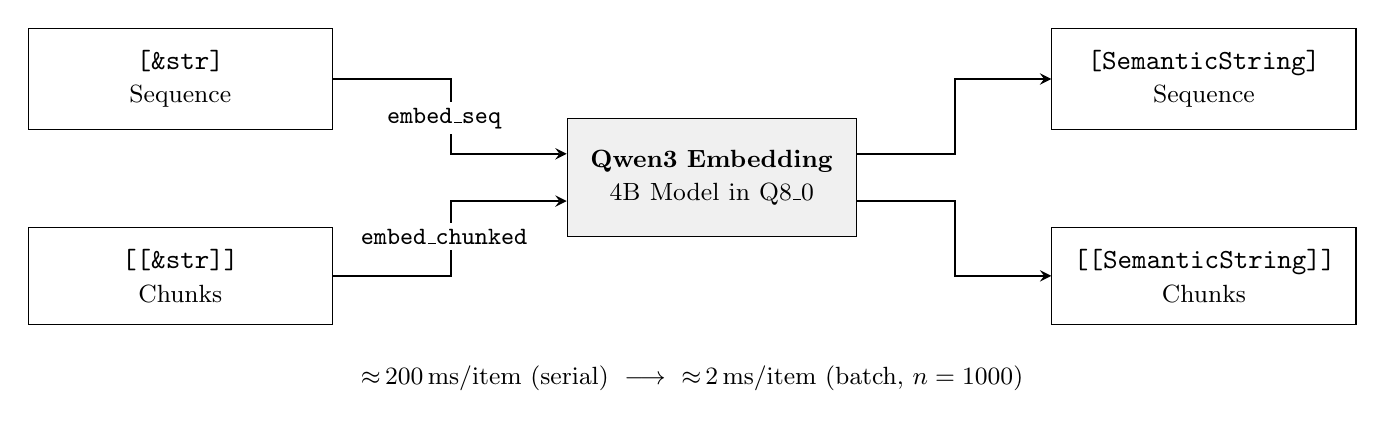
\begin{tikzpicture}[
    box/.style={draw, rectangle,
                minimum width=3.5cm, minimum height=0.9cm,
                text width=3.3cm, align=center, inner sep=8pt},
    gpu/.style={draw, rectangle,
                minimum width=3.5cm, minimum height=1.5cm,
                text width=3.25cm, align=center, inner sep=6pt, fill=gray!12},
    arr/.style={->, thick, >=stealth}
  ]
    \node[gpu] (model) at (6.75,0.75)
    {{\small\textbf{Qwen3 Embedding}}\\{\small 4B Model in Q8\_0}};

    \node[box] (seq_in)  at (0,2)    {\texttt{[\&str]}\\{\small Sequence}};
    \node[box] (seq_out) at (13,2)   {\texttt{[SemanticString]}\\{\small Sequence}};

    \node[box] (chunk_in)  at (0,-0.5)  {\texttt{[[\&str]]}\\{\small Chunks}};
    \node[box] (chunk_out) at (13,-0.5) {\texttt{[[SemanticString]]}\\{\small Chunks}};

    \draw[arr] (seq_in.east)   -- ++(1.5,0) |- ([yshift=3mm]model.west);
    \draw[arr] (chunk_in.east) -- ++(1.5,0) |- ([yshift=-3mm]model.west);

    \node[font=\small, fill=white, inner sep=2pt] at (3.35, 1.5)  {\texttt{embed\_seq}};
    \node[font=\small, fill=white, inner sep=2pt] at (3.35, 0.0) {\texttt{embed\_chunked}};

    \draw[arr] ([yshift=3mm]model.east)  -- ++(1.25,0) |- (seq_out.west);
    \draw[arr] ([yshift=-3mm]model.east) -- ++(1.25,0) |- (chunk_out.west);

    \node[align=center, font=\small] at (6.5,-1.8)
      {$\approx$\,200\,ms/item (serial)
       $\;\longrightarrow\;$
       $\approx$\,2\,ms/item (batch, $n = 1000$)};
  \end{tikzpicture}
  \caption{Batch embedding data flow. Inputs are either flat sequences (\texttt{embed\_seq}) or pre-chunked slices (\texttt{embed\_chunked}); the chunked path preserves the original layout for seamless reconstruction. Batch processing reduces per-item embedding time from $\approx$\,200\,ms to $\approx$\,2\,ms.}
  \label{figure:batch-embedding}
\end{figure}

\subsubsection{Wasserstein-Weisfeiler-Leman Kernels}

WWL kernels are used to construct the distance index $d \in \mathcal{D}$
for the $\sigma$ function (see section~\ref{design:selection-function})
by computing schema distance through graph-based distance metrics. The
underlying WWL implementation used by \textsc{Natural} is the reference
implementation of WWL kernels from \citeauthor{WWL}, which is implemented in
Python. Thus \textsc{Natural} can't directly use the WWL implementation
as Rust and Python FFI is not directly possible. In order to buy into the
Python libraries and ecosystem (eg, optimal transport) and utilize the existing
implementation of the WWL kernels, writing a thin layer of Rust bindings around
\citeauthor{WWL}'s implementation was deemed most sensible. Using \texttt{pyo3}
calling Python code is made possible and let's \textsc{Natural} hook into
existing ecosystems where needed. Due to the design laid out in
section~\ref{section:design} the WWL implementation is only needed during
sampling time and not required at runtime as all distances are precomputed and
stored in a distance index, keeping the runtime portability characteristics of
using Rust that were discussed above.

% - Schema similarity using Weisfeiler-Leman graph kernel
% - O(n²) computational complexity for 100+ database schemas
% - Precomputation during initialization vs dynamic updates
% - Node labeling strategy: constraints vs data types hierarchy
% - Distance index caching: initialization time vs query performance

\paragraph{Rust-Python Integration Architecture}

The WWL kernel library used by \textsc{Natural} is implemented using
\texttt{pyo3} around the existing Python \texttt{wwl} library. The Rust
bindings are usable through the \texttt{wwl} crate. The \texttt{WWLKernel}
struct encapsulates the Python module reference and provides type-safe interfaces for
both categorical and continuous propagation modes through respective methods.
Using an existing graph library (\texttt{petgraph}) the complexity of the Rust
bindings could be kept minimal, but required conversion from Rust's
\texttt{petgraph} graph representation to Python's \texttt{igraph} graph
representation. 

\paragraph{Schema Graph Representation}

The \texttt{natural-graphs} library implements the schema graph representation
discussed in section~\ref{design:graph-repr} by parsing SQL statements using the
\texttt{sqlparser} library and constructing an undirected \texttt{petgraph}
graph instance. Nodes represent tables and columns and edges capture foreign
key relationships and column ownership. Node labeling is used to encode schema
constraints hierarchically as outlined in section~\ref{design:graph-repr}.

\paragraph{Propagation Mechanisms}

The \texttt{wwl} crate supports both categorical and continuous Weisfeiler-Leman
propagation schemes. Categorical propagation operates on discrete node labels
through iterative label refinement, suitable for constraint-based schema
comparison. Continuous propagation utilizes node features encoded in matrices,
enabling similarity computation based on quantitative schema properties like
column cardinalities or data type frequencies \citep{WWL}. As \textsc{Natural}
projects the database schema into a graph representation with categorical node
labels, the categorical propagation scheme is used in \texttt{natural-graphs}
to determine schema distance. The \texttt{wwl} bindings allow configuration of
the kernel through the \texttt{KernelConfig} and \texttt{DistanceConfig}
structs, which provide control over the iteration count (which defaults to 3),
sinkhorn approximation settings etc. 

\paragraph{Distance Computation and Caching}

The pairwise Wasserstein distance is computed between the current database
schema and each sample database during sampling phase. The distance index is
a \texttt{HashMap} of a sample database name to it's distance to the current
database \textsc{Natural} is running on. Caching of this computation is an
efficient strategy to minimise runtime inference time as the distance index is
static as long as database schemas are not mutated. \textsc{Natural} is storing
JSON-serialized distance indices in \texttt{Vector} for fast distance lookups
at runtime. This design prevents the computational cost of WWL distance
computations from affecting inference, reducing runtime schema comparison to
constant-time lookups for all previously indexed database combinations that
were known during sampling time. Given that the set of sample database and
target databases are usually fixed, the distance lookup becomes negligible in
terms of computational cost.

\paragraph{Integration with Example Selection}

The WWL kernel is integrated in the sampling phase, where distance indices are
computed and cached. Furthermore during example selection ($\sigma$) the
cached distance index is loaded from \texttt{Vector} for distance lookups.

The distance index is used for weighting the schema compatibility in the
selection algorithm (see section~\ref{design:selection-function}) to balance
structural similarity against question-level semantic relevance for improved
in-context learning effectiveness.

\subsection{Benchmarking Infrastructure}\label{impl:benchmark}

\textsc{Natural}'s benchmarking infrastructure is implemented in
\texttt{natural-benchmark}. This benchmarking infrastructure is enabling the
development, verification and ultimately deployment of \textsc{Natural}
pipeline. This section focuses on the respective benchmarking infrastructure
development, performance optimizations that were required and engineering
challenges encountered. 

Whilst \textsc{Natural}'s benchmarking infrastructure is not part of the core
pipeline, it helps to develop and test hypotheses for extensions or design
changes confidently, compare performance across pipeline versions, models and
understand the benchmark performance.

\subsubsection{Execution-Based Evaluation System}

The \texttt{natural-benchmark} CLI evolves around the concept of executions
which are single benchmark runs against a specific benchmark dataset
(defaulting to \textsc{Spider}). An execution is the set of tests that have
been executed using a version of \textsc{Natural} against a benchmark. The
interface of \texttt{natural-benchmark} offers multiple options to create
executions and subsequentlty understand \textsc{Natural}'s performance:

\begin{enumerate}
    \item Running new benchmarks via: \\ \texttt{natural-benchmark new}
    \item Continuing a halted execution via: \\ \texttt{natural-benchmark continue --execution <id>}
    \item Comparing performance on previous (partial) executions via: \\ \texttt{natural-benchmark compare-to --previous <id>}
    \item Computing statistics on past executions via: \\ \texttt{natural-benchmark stats --execution <id>}
\end{enumerate}

While benchmarking \texttt{natural-benchmark} maintains a local SQLite database
maintaining a history of past performance, pipeline failures etc. for future
introspection as well as comparison of approaches.

\subsubsection{Cross-Dataset Validation}

In order to measure the performance of \textsc{Natural} against multiple
benchmarking datasets, the benchmarking and execution system in
\texttt{natural-benchmark} must be generalize across one dataset. The
benchmarking setup achieves this through a set of rust traits (eg, type
characteristics) to model benchmarking datasets. 

The traits \texttt{Benchmark}, \texttt{BenchmarkDatabase} and
\texttt{BenchmarkTest} allow to abstract the file system layout of different
evaluation datasets. Thus when implementing benchmark support against
\textsc{Spider} the implementation absatracts the fact that \textsc{Spider} is
using SQLite for test databases, and uses a JSON file to store the questions.
The file system layout of \textsc{Spider} and \textsc{Bird} is largely similar.

This abstracted benchmarking system (see \ref{appendix:benchmark-traits})
allows integrating further benchmarks in the future (eg, \textsc{Spider2} which
relies on cloud databases like Snowflake) while maintaining the same ergonomics
and tooling across benchmark datasets (eg, recording and indexing all test
executions in a local database, recording pipeline logs etc). 

\subsubsection{Metric Computation}

The benchmarking infrastructure computes the two metrics \textsc{Execution
Accuracy} and \textsc{Exact Match} found in prevalent benchmark leaderboards
(eg, \textsc{Spider} and \textsc{Bird}) through a Rust port of the Python
reference implementation found in \textsc{Spider}. \textsc{Spider} determines
the \textsc{Execution Accuracy} by comparing the result sets of two queries
based on possible row and column permutations as well as optional order
sensitivity. The \textsc{Exact Match} metric is determined by exact equivalence
of the ground truth query $\omega_{ground}$ and the candidate query $\omega$.

\subsubsection{Benchmarking Challenges}

Two primary issues emerged while developing the benchmarking infrastructure for
\textsc{Natural}:

While loading result sets from the provided test database, a faulty
code path failed to parse query result with types other than
\texttt{Text}. This caused empty result sets to be returned as query results
from both the ground truth query and the candidate query, resulting in a false
positive, skewing the \textsc{EA} metric significantly upwards.

Furthermore frequent pipeline failures of \textsc{Natural} made it hard to get
compute reliable performance metrics as context window constraints, out
of memory issues and CUDA issues caused a significant number of test
cases to fail, making subsequently computed metrics unreliable as only
a subset of the dataset was included in the results.

\subsection{Engineering Challenges and Lessons Learned}

The implementation approach of \textsc{Natural} highlighted significant
challenges in terms of practicability that were independent of the algorithmic
design and theoretical problems. While \textsc{Natural} turned out to
demonstrate the approaches recommended in the system design section, the
development process was significantly slowed down due to constrained hardware
availability, technology stack decisions and research methodology. The overall
system architecture turned out positive, but the timeline was noticeably expanded.

This section reflects on the most impactful challenges that were encountered
during the implementation of \textsc{Natural} and analyzes how hardware
limitations influenced design decisions, confidence in the performance of
\textsc{Natural} and the overall impact on development velocity. These insights
are transferable beyond \textsc{Natural} and are applicable to any
production-grade implementation of research algorithms.

\subsubsection{Hardware Constraints and Development Velocity}

Likely the most significant circumstance that affected development velocity was
the constrained access to high performance hardware. The hardware available
during development time was the RTX 3090 with 24GB of VRAM. This limitation
fundamentally shaped the development process and research methodology as the
iteration speed was severely slowed down.

\paragraph{Benchmarking and Evaluation Bottlenecks}

A full benchmark execution of \textsc{Natural} against the \textsc{Spider} test
dataset required around 12-36 hours depending on the number of
candidates generated and refinement algorithm used during the benchmark. 
This made continuous validation during development a non trivial task,
requiring extensive evaluation phases between times of active development.

Testing new hypotheses, validating algorithmic changes, experimenting with the
implementation approaches, comparing different configurations and sampling
strategies therefore became multi-week processes rather than the rapid
iteration typically desired in research environments.

The prolonged evaluation cycles created a cascading effect on development
velocity. Rather simple adjustments that would normally be validated within
hours required days of computational time, effectively preventing what should
have been normal experimentation. The hardware constraints forced a rather
conservative approach to experimentation, where each change needed to be
carefully considered before committing to multiple days of benchmarking.

\paragraph{Memory Management and CUDA Issues}

Frequent CUDA out-of-memory (OOM) errors made the evaluation interpretation non
trivial as accuracy scores became inaccurate due to pipeline failures. This
persisted as a second development challenge throughout the implementation
phase. These memory exhaustion issues occurred rather unpredictable during both
development and benchmarking, depending on the database schema and question
asked. As \textsc{Natural} uses a code representation prompt, the database
schema is inlined into the prompt during inference. If \textsc{Natural} is
executed against large databases, even with schema subsetting, the context
window can be exceeded or the KV-Cache can exhaust the rest of the available
GPU memory (typically around 2-4 gigabytes) after models have been loaded. This
required extensive trial-and-error debugging to identify the root causes and
implement workarounds. 

\subsubsection{Technology Stack Trade-offs}

During the implementation of \textsc{Natural}, several critical technology
stack decisions fundamentally impacted both development velocity and the
final system characteristics. The two most consequential decisions were the
choice of programming language and the model deployment strategy, each
presenting distinct trade-offs between research efficiency and production
readiness.

\paragraph{Programming Language: Rust vs Python}

The decision to implement \textsc{Natural} in Rust rather than Python
represents perhaps the most impactful architectural choice made during the
implementation phase. Choosing Rust presented the opportunity to port the
research system into production environments soon after, but came at the cost
of having to port existing benchmarking infrastructure and not being able to
exactly reuse the inference code used by \textsc{OmniSQL}. This decision
significantly increased implementation time, likely doubling the development
effort compared to what would have been required in Python. Using Python would
have provided immediate access to existing machine learning infrastructure and
could have leveraged existing implementations by previous researchers directly
in the implementation of \textsc{Natural}. The rather mature Python ecosystem
for NLP and ML would have eliminated the need to develop abstractions for model
inference, vector database operations, and benchmark evaluation.

However, the Rust implementation as is provides significant benefits for production
deployment and system integration. The resulting system can be embedded
directly into database systems such as PostgreSQL through extensions,
providing a path toward true production deployment that would be impractical
with Python. The ability to compile an entire NL2SQL system into a single,
standalone binary offers superior portability characteristics.

\paragraph{Model Deployment: Local vs Cloud-Based Inference}

Using local and open source models reemphasized the limited local hardware
access as using a cloud provider like OpenAI or Anthropic for inference would
have significantly speeded up the benchmarking time. As a primary research goal
of this thesis is to explore the open source capabilities of NL2SQL systems,
choosing a proprietary inference service was deemed unviable.

\paragraph{Integration Complexity and Ecosystem Maturity}

The machine learning ecosystem of Rust proved to be significantly less mature
than anticipated, requiring extensive custom development and research for
functionality that would be available off-the-shelf in prevalent Python packages.
The integration with Python libraries for specialized components like the
Wasserstein-Weisfeiler-Leman kernels required rather complex FFI code using
\texttt{pyo3}, further adding architectural complexity and potential stability
concerns.

Despite these challenges, the resulting architecture demonstrates that multi
language approaches can be viable when different components have distinct
requirements. The Python integration was isolated to the sampling phase,
preserving the runtime portability characteristics of the core Rust
implementation while still leveraging existing, specialized libraries where
appropriate.

\subsubsection{Lessons Learned and Future Recommendations}

The implementation of \textsc{Natural} showed multiple practical challenges
associated with researching and implementing NL2SQL systems. The approach used
in this thesis highlights several areas of consideration for future research
projects in this field.

\paragraph{Hardware Infrastructure Requirements}

Research of modern NL2SQL systems induces steep hardware requirements onto
researchers. Priority should be given to securing access to significantly
powerful hardware and computing infrastructure for faster iteration cycles.

While the 24GB VRAM constraint of the RTX 3090, may be reasonable for most
consumer grade applications, it proved insufficient for efficient iteration in
this field, especially given the involvement of LLMs. Systems with 48GB+ of
VRAM would have enabled the usage of larger, more capable models without the
quantization compromises that may impact system accuracy. More modern hardware
(even on the consumer grade level) would allow for a tremendous benchmarking
speed up (eg, using a 5090 would have resulted in nearly 200\% increase in
speed).

More critically, the availability of multiple GPUs would have enabled parallel
experimentation and benchmarking, which could transform multi-day iteration
cycles into more manageable timeframes. The ability to run concurrent
experiments with different configurations, models, or algorithmic approaches
would dramatically accelerate the research and development process and enable
more thorough experimental validation.

\paragraph{Technology Stack}

The implications of choosing between Rust and Python underlines the importance
of technology choices with research goals and time constraints. For pure
research projects focused on algorithmic development and experimentation,
Python's ecosystem and extensive existing implementations provide clear
advantages that likely outweigh the deployment benefits of compiled languages
like Rust.

However, for projects with a clear path to production deployments or those
intended to bridge academic research with real-world applications, the
additional development overhead of systems programming languages like Rust can
be justified. Overall, hardware availability weighs significantly more than
language choices when it comes to the implementation timeline.

Future implementations in this field should likely consider a two-staged
approach: prototyping and algorithm validation in Python to leverage existing
tools and accelerate iteration, followed by a production port in a systems
language like Rust once the algorithmic approach is validated and stable.

\paragraph{Development Methodology Recommendations}

The challenges encountered suggest several methodological improvements for
future projects:

Implementing benchmarking and validation infrastructure early in the
development process is crucial when doing algorithmic development to gain an
understanding of the relative improvement or setback of different approaches.

Establishing performance baselines and using incremental validation procedures
can help ensure that development effort is focused on improvements that in fact
improve performance.

The long running benchmarks made it difficult to validate whether
individual changes were beneficial, leading to uncertainty about the
effectiveness of specific optimizations. In situations with highly constrained
compute resources, a representative subset of prevalent benchmarking datasets
like \textsc{Spider} and \textsc{Bird} may be defined to determine the relative
improvement between approaches before executing a full benchmark run.

Finally, maintaining detailed logs and metrics throughout the development
process showed to be crucial when unexpected errors occur. Identifying root
causes of pipeline failures was rather trivial due to having an advanced
benchmarking setup with log collection.

\paragraph{Research Impact and Production Readiness}

Despite all challenges encountered in the implementation phase, the Rust
implementation of \textsc{Natural} demonstrate that it is possible to port
research algorithms from academic environments into production-ready systems.
The resulting implementation provides a strong foundation for real-world
deployments in database environments, which would be significantly more
challenging with a Python-based research prototype.

This production readiness ensures that all algorithmic contributions can have
practical impact beyond pure academic evaluation, potentially influencing how
NL2SQL systems are deployed in real database environments. A simple
recommendation between research velocity and production readiness can not be
given as it ultimately depends on the intended impact and longevity of the
research contributions and implementation.
